\subsection{\acs{NEF}}
\label{chap:proposal:exposure:nef}

In the context of the proposed testbed, three \acs{NEF} northbound \acsp{API} are considered to address distinct, yet complementary aspects of network application behavior. The \textit{AsSessionWithQoS} \acs{API} targets \acs{QoS} control, providing applications with the means to establish and manage application sessions with specific \acs{QoS} profiles designed to guarantee, for example, specific bandwidth or latency requirements~\cite{ETSI_TS_129_122_V18_8_0}. This supports use cases that depend on predictable network behavior, letting applications programmatically request connectivity with specific characteristics, such as guaranteed uplink throughput or traffic priority, without human intervention. Notable examples include \acs{PPDR} applications needing temporary network resources for sporadic emergencies, and real-time video applications requiring low latency (e.g. eHealth) or support for large audiences (e.g. live broadcasting).

However, passively relying on the \acs{QoS} session established via this \acs{API} is not sufficient, as undetected violations of network requirements directly risk the correct functioning of the Network Application. Therefore, there is a clear need for a mechanism capable of actively monitoring the network and detecting any violations of the defined \acs{QoS} in real time. The \textit{AnalyticsExposure} \acs{API} addresses this problem giving developers the ability to query network analytics and subscribe to analytics notifications~\cite{ETSI_TS_129_522_V18_11_0}, allowing applications to monitor network metrics and adapt their behavior according to the observed conditions.

\acs{QoS} violations and changes in network conditions are not the only criteria that can require adaptive application behavior. According to its use case, the network application may need to be notified about specific events in the \acs{3GPP} network, completely unrelated to \acs{QoS}, such as an \acs{UE} becoming unreachable or changing location. The \textit{MonitoringEvent} \acs{API} was designed to create and manage such monitoring event subscriptions~\cite{ETSI_TS_129_122_V18_8_0}, covering events such as location reporting, loss of connectivity, \acs{UE} reachability and roaming status.

These common events can trigger different operations depending on the vertical and application scenario. For example, a \acs{TL} platform may use location updates to trigger \acs{QoS} adjustments as a teleoperated vehicle enters geofenced zones~\cite{NextGenConnectivityDynamicQoS}. In this way, monitoring events complement the \textit{AsSessionWithQoS} \acs{API} by enabling applications to adapt their requested \acs{QoS} in response to changes in \acs{UE} state.

The testbed requires all three \acsp{API} to support the envisioned network application behavior. In the remainder of this section, a closer look is taken at the \textit{AsSessionWithQoS} and \textit{AnalyticsExposure} \acsp{API}, which will be addressed in the next chapter.

\subsubsection{AsSessionWithQoS \acs{API}}
\label{chap:proposal:exposure:nef:AsSessionWithQoS}

The \textit{AsSessionWithQoS} \acs{API}, originally defined in \acs{3GPP} TS~29.122~\cite{ETSI_TS_129_122_V18_8_0}, allows applications to configure sessions indicating the desired level of \acs{QoS} for a given traffic flow. Through notifications, the \acs{API} also informs the application whether the requested \acs{QoS} can be enforced in the network.

The interaction is initiated when the \acs{AS}/\acs{AF} (e.g. a network application) submits an HTTP POST request to the \acs{NEF}, carrying an \texttt{AsSessionWithQoSSubscription} resource body~\cite{ETSI_TS_129_122_V18_8_0}. This body comprises an extensive set of parameters whose presence is governed by conditional rules, depending on the remaining payload content and on the \acs{API} features supported by the \acs{5GC}. Rather than covering all of these parameters, this section focuses on the attributes that express the desired \acs{QoS} configuration.

These include the target \acs{UE}, typically identified by its \acs{IP} or \acs{MAC} address, although groups of \acsp{UE} (\texttt{extGroupId}) or a subscription identifier such as the \ac{GPSI} may also be used when the corresponding features are supported. The traffic flow subject to \acs{QoS} treatment is then described as an \acs{IP} flow (\texttt{flowInfo}) or an Ethernet flow (\texttt{ethFlowInfo}), in accordance with the type of address provided.

The requested \acs{QoS} for that flow can be defined through the \texttt{qosReference} attribute, which references pre-defined \acs{QoS} information (e.g. \acs{QCI}/\acs{5QI} and associated parameters defined by the operator), optionally complemented by \texttt{altQoSReferences}, an ordered list of alternative references ranked by priority. Alternatively, a list of alternative service requirements (\texttt{altQosReqs}) can also be specified, each containing an individual set of \acs{QoS} parameters, namely the guaranteed bandwidth in uplink (\texttt{gbrUl}) and downlink (\texttt{gbrDl}), the packet delay budget (\texttt{pdb}) and the packet error rate (\texttt{per}). Finally, the attribute \texttt{notificationDestination} supplies the \acs{URL} at which the application will receive all notification events.

The specification further defines attributes such as usage thresholds (\texttt{usageThreshold}), \acs{QoS} signalling control (\texttt{disUeNotif}), and requirements for time sensitive communications (\texttt{tscQosReq}), which are beyond the scope of the targeted used cases. It also supports \acs{QoS} monitoring, through which the application subscribes to the \texttt{QOS\_MONITORING} event to receive measurements on the established flow. These measurements are limited to packet delay (\texttt{qosMonInfo}), data rate (\texttt{qosMonDatRate}) and congestion information (\texttt{qosMonConReq}), which are usually not covered nor utilized in the examples found throughout the literature.

Following the creation request, the \acs{NEF} maps the supplied \acs{QoS} references/parameters and coordinates with the \acs{PCF} to enforce the \acs{QoS} policy. As previously mentioned, the \texttt{notificationDestination} \acs{URI} included in the subscription body designates the callback endpoint to which the \acs{NEF} will deliver notifications. These notifications are conveyed through the \texttt{UserPlaneNotificationData} payload specifying a list of event reports for the user plane. From the possible notification event types, the testbed would rely on \texttt{SUCCESSFUL\_RESOURCES\_ALLOCATION} and \texttt{FAILED\_RESOURCES\_ALLOCATION}, which indicate whether the resources required by the requested \acs{QoS} could be allocated in the network. Other events of note for the \acs{QoS} use case include \texttt{QOS\_GUARANTEED} and \texttt{QOS\_NOT\_GUARANTEED}, which indicate whether the network is currently able to meet the \acs{QoS} targets, \texttt{QOS\_MONITORING}, which delivers the \acs{QoS} monitoring measurements, and \texttt{USAGE\_REPORT}, which provides consumption information according to the \texttt{usageThreshold} provided in the request.

\begin{figure}[htpb]
    \centering
    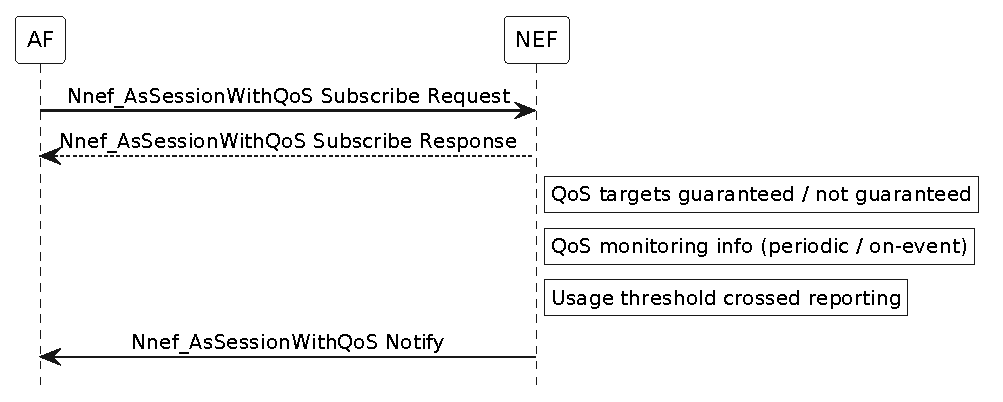
\includegraphics[width=1\linewidth]{figs/plantuml/as-session-with-qos-proposal-flow.pdf}
    \caption{Information flow for the \textit{AsSessionwithQoS} \acs{API}}
    \label{fig:flow:AsSessionWithQoSAPI}
\end{figure}

Figure \ref{fig:flow:AsSessionWithQoSAPI} highlights the described information flow for the \textit{AsSessionWithQoS} \acs{API}, obtained from the overall information flow described in TS 23.502~\cite{3GPP-23.502} and scoped to the interactions between the \acs{AF} and the \acs{NEF}, omitting internal network procedures beyond the \acs{NEF} (e.g. with the \acs{PCF}). Through this procedure, the \acs{NEF} \textit{AsSessionWithQoS} \acs{API} represents the primary programmable point in the testbed, enabling network applications to express and enforce \acs{QoS} requirements and the network conditions required to support the specific demands of each network application use case.


\subsubsection{AnalyticsExposure \acs{API}}
\label{chap:proposal:exposure:nef:AnalyticsExposure}

The \textit{AnalyticsExposure} \acs{API}, defined in \acs{3GPP} TS~29.522~\cite{ETSI_TS_129_522_V18_11_0}, allows an \acs{AF} to obtain analytics information about the network. Analytics can be retrieved through one-time fetch requests or through subscriptions, in which the \acs{NEF} notifies the \acs{AF} periodically or when specific conditions are met. Within the testbed, this \acs{API} would be the northbound interface through which the network metrics described in Section~\ref{chap:proposal:observability}, are made available to network applications.

In the \acs{5G} System, network analytics are natively produced by the \acs{NWDAF}~\cite{ETSI_TS_123_288_V18_11_0}. This function collects data scattered across multiple network functions, such as the \acs{AMF}, \acs{SMF} and \acs{UPF}, and derives new analytics from it, in the form of statistics or predictions. The \acs{NEF} then exposes these analytics to external consumers through the \textit{AnalyticsExposure} \acs{API}. However, although the specification defines the \acs{NWDAF} as the source from which the \acs{NEF} obtains analytics~\citep{ETSI_TS_123_288_V18_11_0, ETSI_TS_129_522_V18_11_0}, the \acs{AF} interacts exclusively with the \acs{NEF} and its standardized data model, making the origin of the analytics transparent to the application. The \acs{NEF} could therefore expose analytics obtained through alternative means, such as the analysis of raw \acs{IP} traffic, as long as they follow the standardized data model. This is particularly relevant for the testbed, as it would allow network application requirements and behavior to be validated without depending on an \acs{NWDAF}.

The specification defines a set of analytics events, each associated with its own analytics payload, as listed in Table~\ref{tab:proposal:exposure:nef:analytics_events}. For instance, \texttt{DN\allowbreak\_PERFORMANCE} reports the data rate, packet delay and packet loss between \acsp{UE} and an application server, while \texttt{UE\allowbreak\_COMM} characterizes the communication of \acsp{UE} with a given application, including the exchanged traffic volume.

\begin{table}[htbp]
    \centering
    \renewcommand\tabularxcolumn[1]{m{#1}}
    \begin{tabularx}{\textwidth}{|
        >{\RaggedRight\arraybackslash}m{\widthof{\texttt{NETWORK\_PERFORMANCE}}}|
        >{\RaggedRight\arraybackslash}X|}
        \hline
        \textbf{Analytics Event} & \textbf{Description} \\
        \hline
        \texttt{UE\_MOBILITY} & Location and mobility patterns of \acsp{UE}, such as tracking areas, cells or geographical coordinates where \acsp{UE} stay over time and their direction \\
        \hline
        \texttt{UE\_COMM} & Communication patterns of \acsp{UE}, such as periodicity, duration and uplink/downlink traffic volume \\
        \hline
        \texttt{ABNORMAL\allowbreak\_BEHAVIOR} & Identifies a group of \acsp{UE} or a specific \acs{UE} with abnormal behavior, e.g. being misused or hijacked \\
        \hline
        \texttt{CONGESTION} & User data congestion in a given area, or in the area where a given \acs{UE} is located \\
        \hline
        \texttt{NETWORK\allowbreak\_PERFORMANCE} & \acs{gNB} status and resource usage, communication and mobility performance, and number of \acsp{UE} in an area of interest \\
        \hline
        \texttt{QOS\allowbreak\_SUSTAINABILITY} & Statistics on past \acs{QoS} changes or likelihood of future \acs{QoS} changes in a given area \\
        \hline
        \texttt{DISPERSION} & Locations or network slices where \acsp{UE} disperse most of their data volume and session transactions, expressed as the percentage of activity generated at each location or slice\\
        \hline
        \texttt{DN\allowbreak\_PERFORMANCE} & User plane performance, namely the average and maximum traffic rate and packet delay, and average packet loss rate \\
        \hline
        \texttt{SERVICE\allowbreak\_EXPERIENCE} & Observed service experience of \acsp{UE} in an application or network slice, expressed through the average and/or variance of the observed service mean opinion score \\
        \hline
        \texttt{E2E\allowbreak\_DATA\allowbreak\_VOL\allowbreak\_TRANS\allowbreak\_TIME} & Time to complete the transmission of a specific data volume from the \acs{UE} to the \acs{AF}, or vice versa \\
        \hline
        \texttt{MOVEMENT\allowbreak\_BEHAVIOUR} & Analytics information (statistics or predictions) regarding e.g. the number, direction and velocity of \acsp{UE} during an analytics target period in a target area \\
        \hline
        \texttt{WLAN\allowbreak\_PERFORMANCE} & Quality and performance of the \acs{WLAN} connection of \acsp{UE} according to their location \\
        \hline
        \texttt{NS\allowbreak\_LOAD\allowbreak\_LEVEL} & Load level of a network slice or network slice instance \\
        \hline
        \texttt{RELATIVE\allowbreak\_PROXIMITY} & Relative proximity among a set of \acsp{UE} \\
        \hline
    \end{tabularx}
    \caption{Analytics events defined for the \textit{AnalyticsExposure} \acs{API}~\cite{ETSI_TS_123_288_V18_11_0, ETSI_TS_129_522_V18_11_0}}
    \label{tab:proposal:exposure:nef:analytics_events}
\end{table}

Figure~\ref{fig:flow:AnalyticsExposureAPI} depicts the information flow for both interaction models of the \textit{AnalyticsExposure} \acs{API}, scoped to the interactions between the \acs{AF} and the \acs{NEF}~\cite{ETSI_TS_123_288_V18_11_0, ETSI_TS_129_522_V18_11_0}. In the subscription model, the \acs{AF} specifies the analytics events of interest, optionally restricted to a set of target \acsp{UE} and to event-specific filters, together with the reporting information, such as the notification method, reporting period and maximum number of reports. The reporting information may also delimit the time period to which the analytics refer. While a past period yields statistics on observed conditions, a future period yields predictions, accompanied by a confidence level, provided that the analytics source (e.g. the \acs{NWDAF}) supports them. The request also carries the callback \acs{URI} to which the \acs{NEF} delivers the analytics notifications, according to the requested reporting information. In the fetch model, the \acs{AF} requests a single analytics event, characterized in the same way, and the analytics are returned directly in the response.

\begin{figure}[htpb]
    \centering
    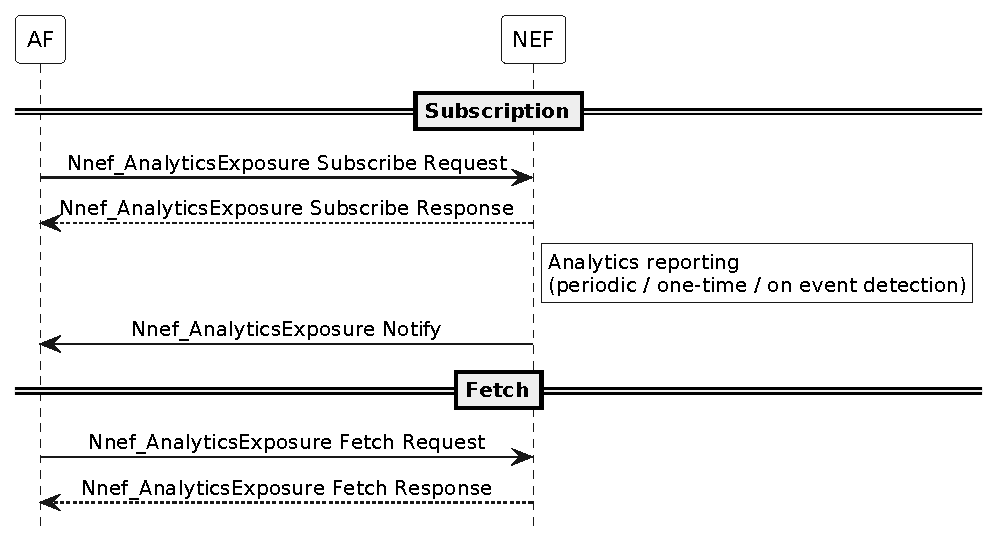
\includegraphics[width=1\linewidth]{figs/plantuml/analytics-exposure-proposal-flow.pdf}
    \caption{Information flow for the \textit{AnalyticsExposure} \acs{API}}
    \label{fig:flow:AnalyticsExposureAPI}
\end{figure}

These analytics events must be integrated with the testbed's monitoring capabilities. This way, network conditions, observed by a monitoring framework, can be exposed through the \textit{AnalyticsExposure} interface and delivered to vertical applications as they change, without the applications continuously polling the network.

In this role, the \acs{API} acts as the bridge between internal network observability and the network application layer, allowing (i) applications to adapt their behavior to the observed, and possibly future, network conditions and (ii) clients to obtain assurance that the network delivers the performance expected for their slice or \acs{QoS} session. Ultimately, the exposed analytics also support the validation of the network application's behavior against its declared requirements, discerning degraded network conditions from bad application logic.
